\chapter{Implementation}

% TODO: Mention that we don't implement concurrency or node merges.
% TODO: Mention that we don't actually implement deletes and updates.

% \section{Environment and Tools Used}

\section{System Architecture}
% TODO: Figure from System Architecture

We have implemented our system according to \autoref{fig:db-architecture} in C++. 
In the following, we inspect the particular implementation of each component.

\subsection*{Buffer Manager}
Our buffer manager serves our system with pages, transparently swapping them between memory and external storage.
Upon construction, it receives a \texttt{page\_size} that determines the fixed-sized number of bytes of every page in the system, as well as a \texttt{page\_count} that determines the maximum number of pages that can be buffered in memory.
Each component requests a page with \texttt{fix\_page} returning a buffer frame. 
After operating on the page, the page is released again by calling \texttt{unfix\_page} on the given frame.
The user can pass a boolean flag to indicate whether the page was modified or not.

When fixing a page we can pass a pointer to a \texttt{PageLogic} object.
\texttt{PageLogic} is an abstract class that can be defined by the user to inject user-specific logic into the buffer manager.
This object will be called by the buffer manager when a page is loaded from external storage to memory or evicted from memory.
This allows us to insert user-specific logic, such as invoking the Delta Tree upon eviction, without coupling the two components.

If a page is not already present in the buffer pool, it is loaded from a file from storage. 
If a \texttt{PageLogic} object is injected into the page's corresponding frame, we call it to perform user-specific logic on the loaded page.
When the user unfixes the page again, we keep the page in the buffer pool until it is chosen for eviction.

When the buffer pool is full, our buffer manager selects a page for eviction. 
The eviction strategy is not under inspection in this thesis, therefore we choose a page at random.
Should the page be marked dirty or new, we call the \texttt{PageLogic} object.
Should it return true, we continue writing the page to storage.
Should it return false, we do not continue with the write and simply discard the page.

\subsection*{Slotted Pages}

We store tuples within pages, accessed through the buffer manager.
As shown in \autoref{fig:slotted-page}, a slotted page consists of a header, a slot array and a data segment.
The header contains metadata about the page, such as the number of slots and the pointer to the data segment.
Each slot points to the corresponding tuple data stored in the data segment.
Through this indirection we can accommodate for variable-length tuples \cite{mdbs2024slides}.
Introducing this indirection impacts the cache locality as we need to follow an additional pointer for every comparison.
There are some optimizations, such as storing parts of the key in the slot itself to speed up comparisons \cite{graefe2014memory}.

Each tuple in the system is identified through its unique \ac{TID}.
Each \ac{TID} consists of 8 B, whereas the upper 6 B contain the \ac{PID} and the lower 2 B contain the slot's ID.

When looking up a tuple in the system, we retrieve the corresponding \ac{TID} from the index given the key.
Through the \ac{TID} we can request the corresponding page through the \ac{PID} from the buffer manager.
When loaded into memory, we can access the slot through the slot ID and retrieve the actual tuple data.

When inserting a new tuple, we first need to find an appropriate page to store it in.
If the buffer pool is full, we need to evict a page before we can load a new one.
Once we have a page, we can allocate a slot for the new tuple in the page's slot array and store the tuple data in the data segment.
We then create a new \ac{TID} for the tuple and insert it into the index.

\begin{figure}[htbp]
  \centering
  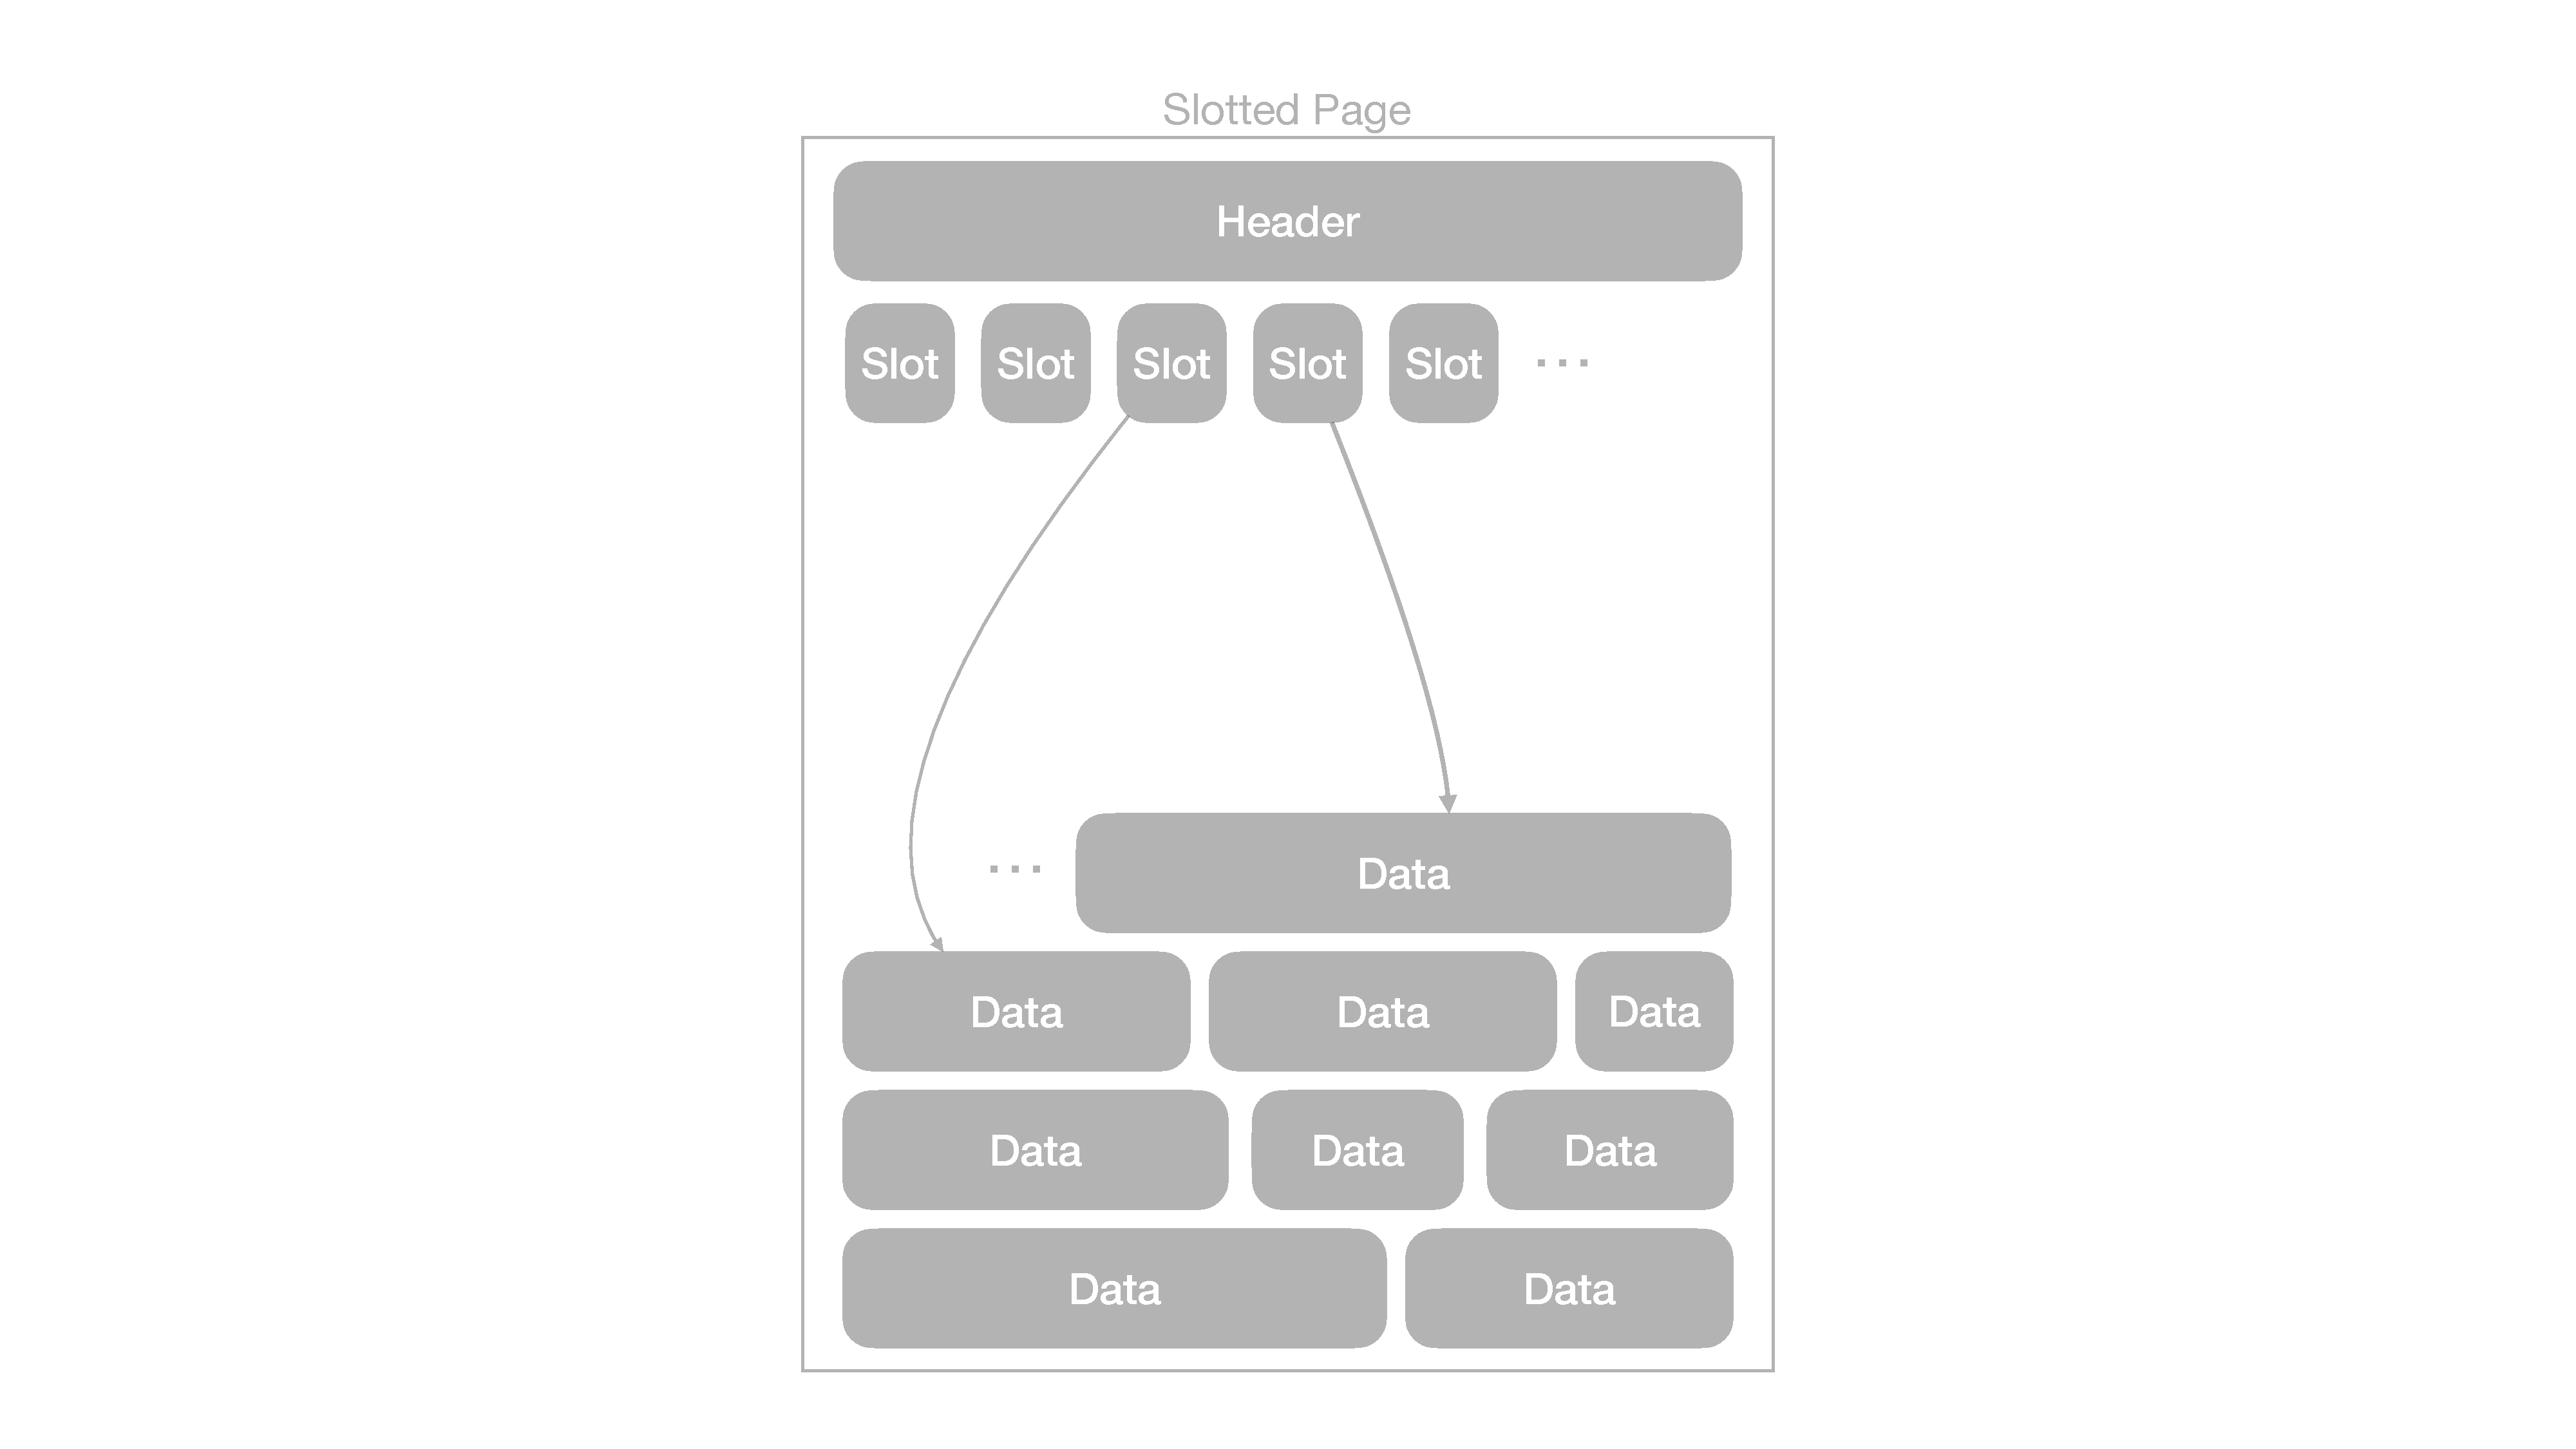
\includegraphics[width=1\textwidth]{figures/slotted_page.pdf}
  \caption{The data layout of a slotted page. The header contains metadata about the page, such as the number of slots and the pointer to the data segment. Each slot points to the actual tuple data stored in the data segment. Tuples can be of variable length and are accessed through their \ac{TID}. Adapted from "Database Systems on Modern CPU Architectures" \autocite{mdbs2024slides}.}
  \label{fig:slotted-page}
\end{figure}

\subsection*{B-Tree}

As shown in \autoref{fig:leaf-node}, each node in our B-Tree is implemented similar to a slotted page to accommodate variable-sized keys and values.
While we depict a leaf node in the figure, inner nodes are implemented similarly.
Leaf nodes store keys and values, whereas inner nodes store keys and \ac{PID}s to child nodes.

We template our B-Tree implementation on the key and value type.
A third boolean template parameter indicates whether we require tracking information to operate a corresponding Delta Tree for this B-Tree instantiation.

\begin{figure}[htbp]
  \centering
  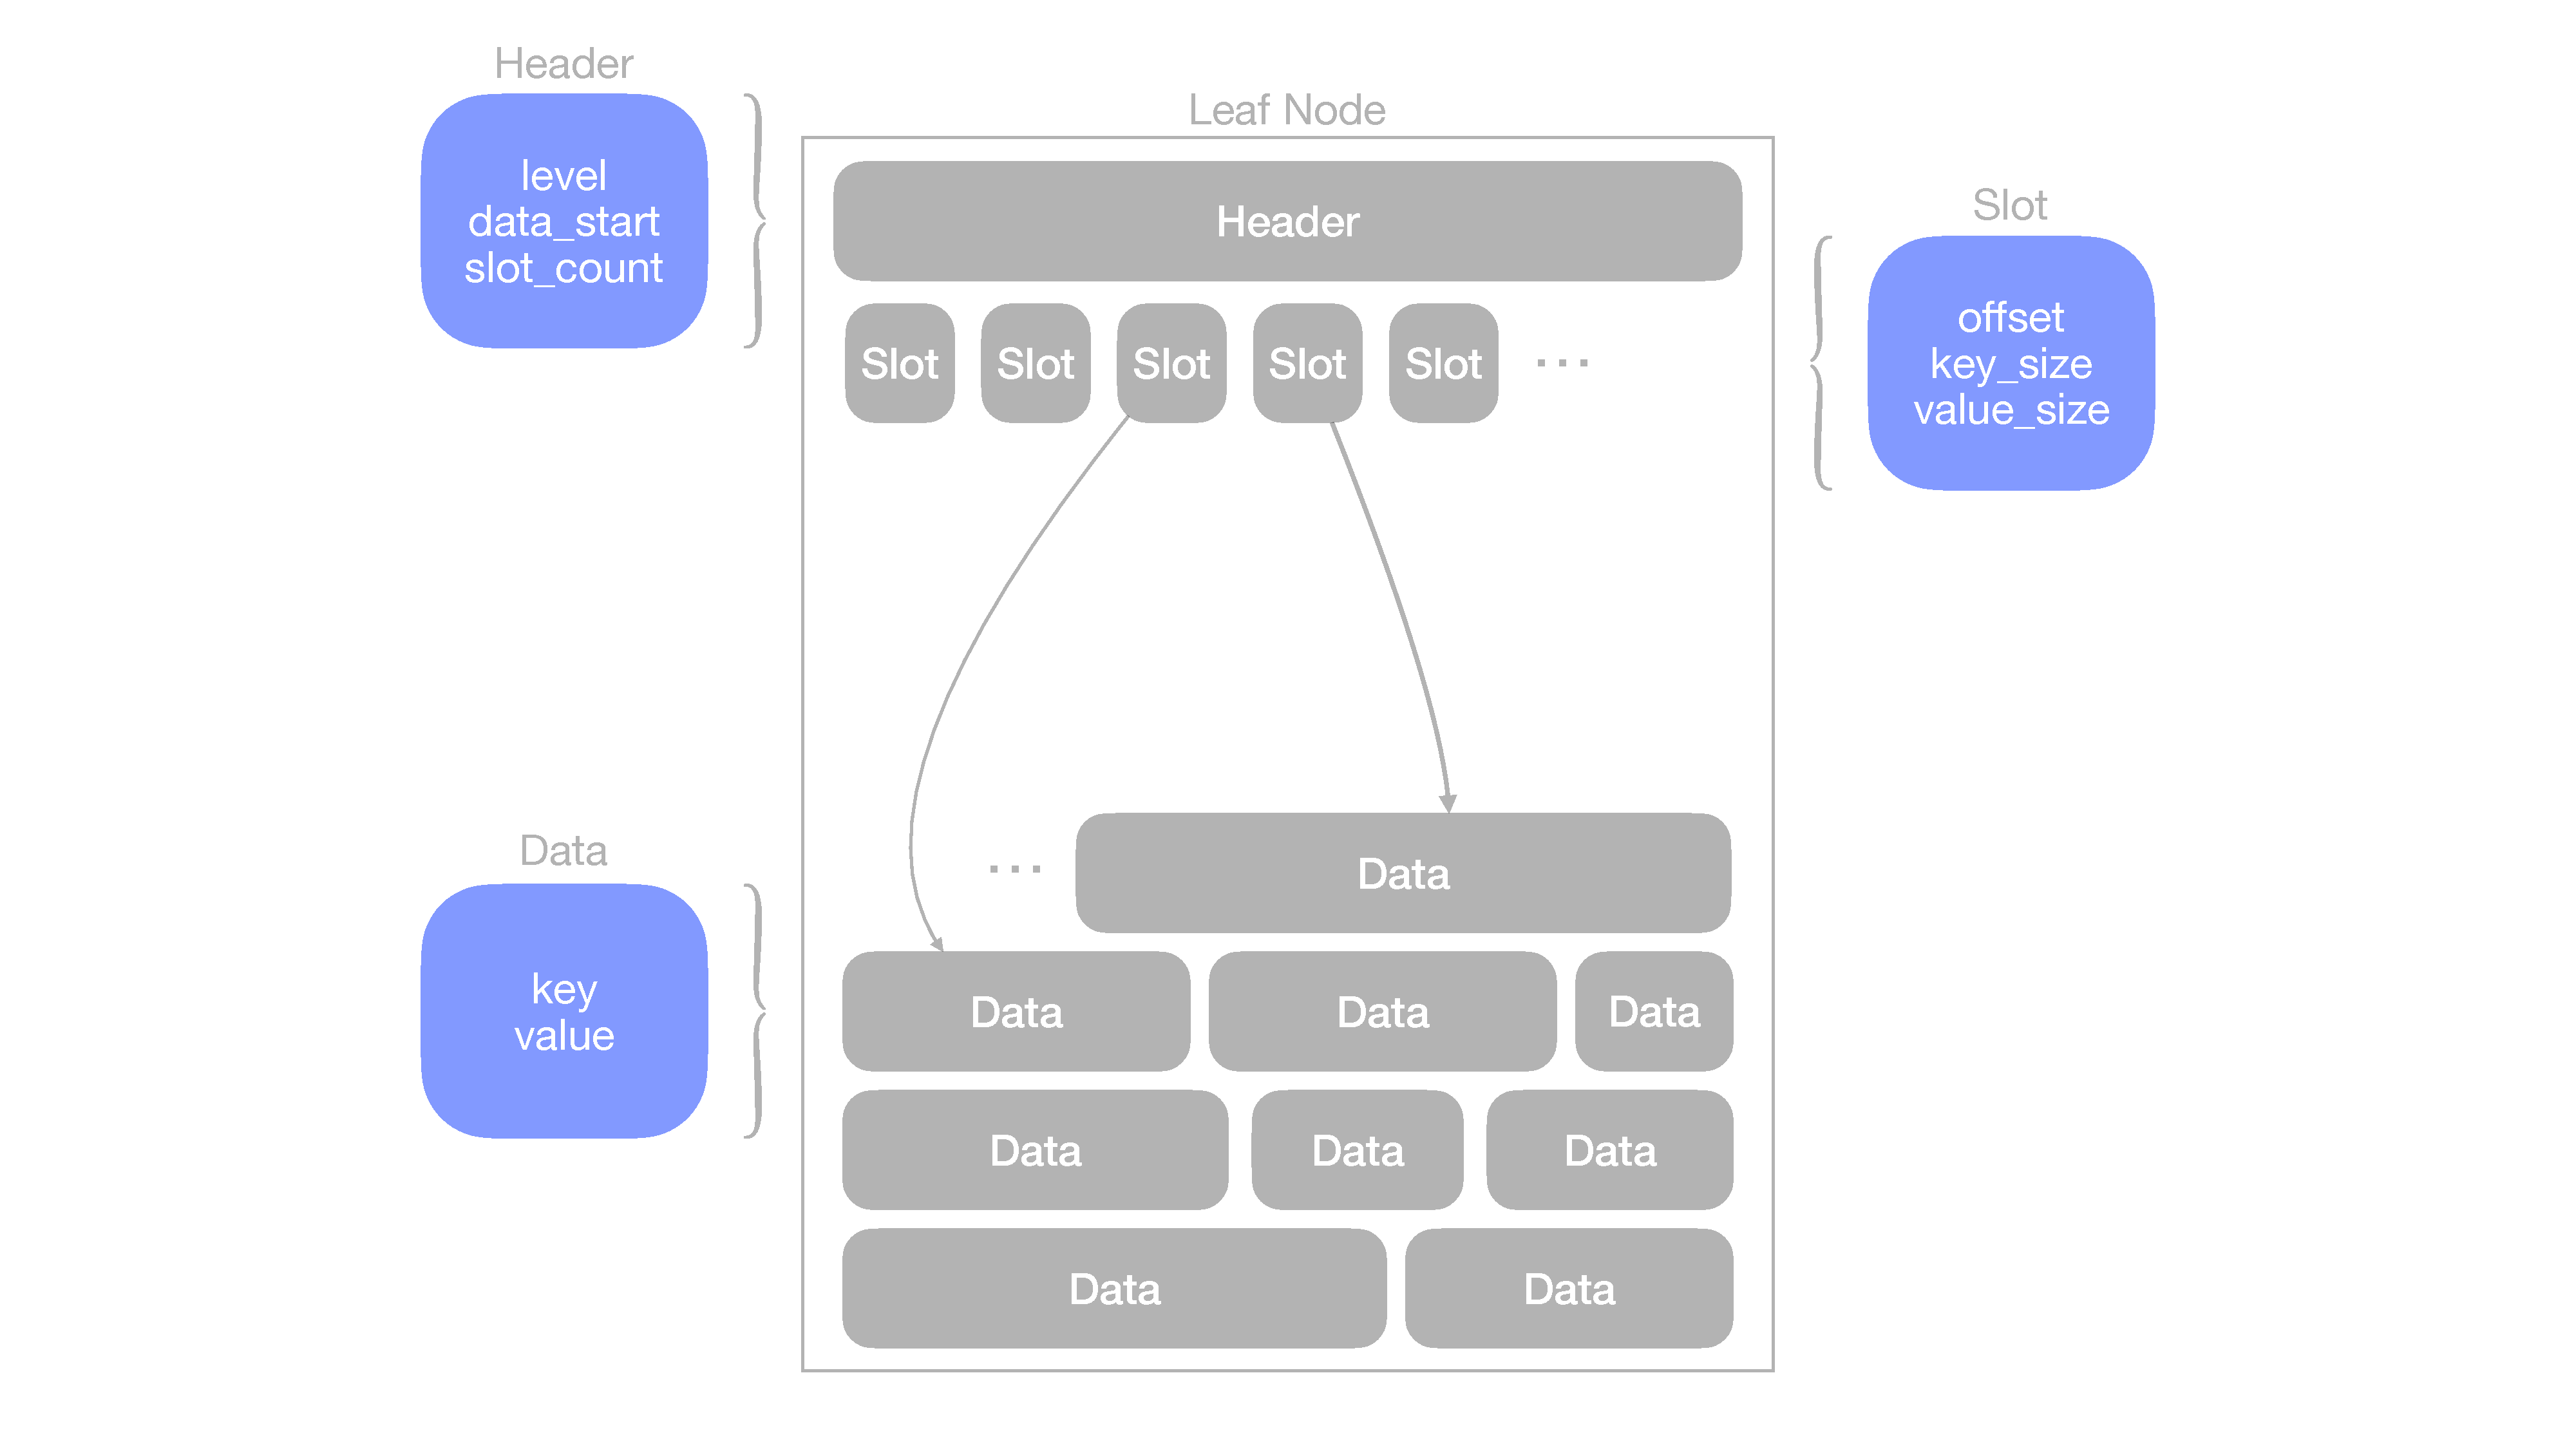
\includegraphics[width=1\textwidth]{figures/leaf_node.pdf}
  \caption{The data layout of a leaf node in the B-Tree supporting variable-sized keys and values. The header contains metadata about the node, such as the level in the tree, the offset to the data segment and the number of slots. The slots point to the actual entries stored in the data segment. The data segment contains the keys and values. Inner nodes store keys and pointers to child nodes. Adapted from "Database Systems on Modern CPU Architectures" \autocite{mdbs2024slides}.}
  \label{fig:leaf-node}
\end{figure}

\subsection*{BBB-Tree}

A BBB-Tree consists of a B-Tree with tracking information and a corresponding Delta Tree.

\subsubsection*{B-Tree with Tracking}
The B-Tree with tracking is a standard B-Tree as described above, but with the addition of tracking changes made to its nodes.
It is templated on the key type \texttt{KeyT} and the value type \texttt{ValueT}, which is always a \ac{TID} in our case.
As described above, we template the B-Tree on a third boolean template parameter.
When set to true, we extend the page header and slots with additional fields to track changes made to the node, as shown in \autoref{fig:b-tree-with-tracking}.

\inlinesection{Header.}
The header is extended by a \texttt{bytes\_changed} field to track the degree of write amplification on the page.
Everytime a change is made to the page, we increase this counter by the number of bytes changed.
When the page is evicted, we can use this information to decide whether to write out the page or not.
However, this is only an approximation of the actual write amplification, as some changes might be overwritten by subsequent changes.
For example, a node split, where we remove half the entries, followed by several insertions can lead to more bytes changed than the actual node size.

\inlinesection{Slots.}
Each slot is extended by a \texttt{state} field to track whether the corresponding entry was \texttt{Unchanged}, \texttt{Inserted}, \texttt{Updated} or \texttt{Deleted} since the last time the page was written to storage.
More specifically, it does not track the change of the entry itself, but rather the change of the entry from the perspective of the node.
For example, if an entry it split off during a node split, the slot is deleted from the perspective of the node.
The entry still exists in the tree, but it is now part of a different node.
To the new sibling node, where we move over the split off entry, the slot is marked as \texttt{Inserted}.
The state machine of the operation state field is shown in \autoref{fig:slot-states} and elaborated in \autoref{sec:algorithms}.

\inlinesection{Buffer Manager Integration.}
Our Delta Tree uses this information to determine which changes to store.
When a B-Tree with tracking enabled, fixes a page through the buffer manager, it injects a \texttt{PageLogic} object into the page's frame.
The buffer manager calls this object later when evicting the node to interact with the Delta Tree to extract deltas and to apply deltas when loading the node from storage again.

\begin{figure}[htbp]
  \centering
  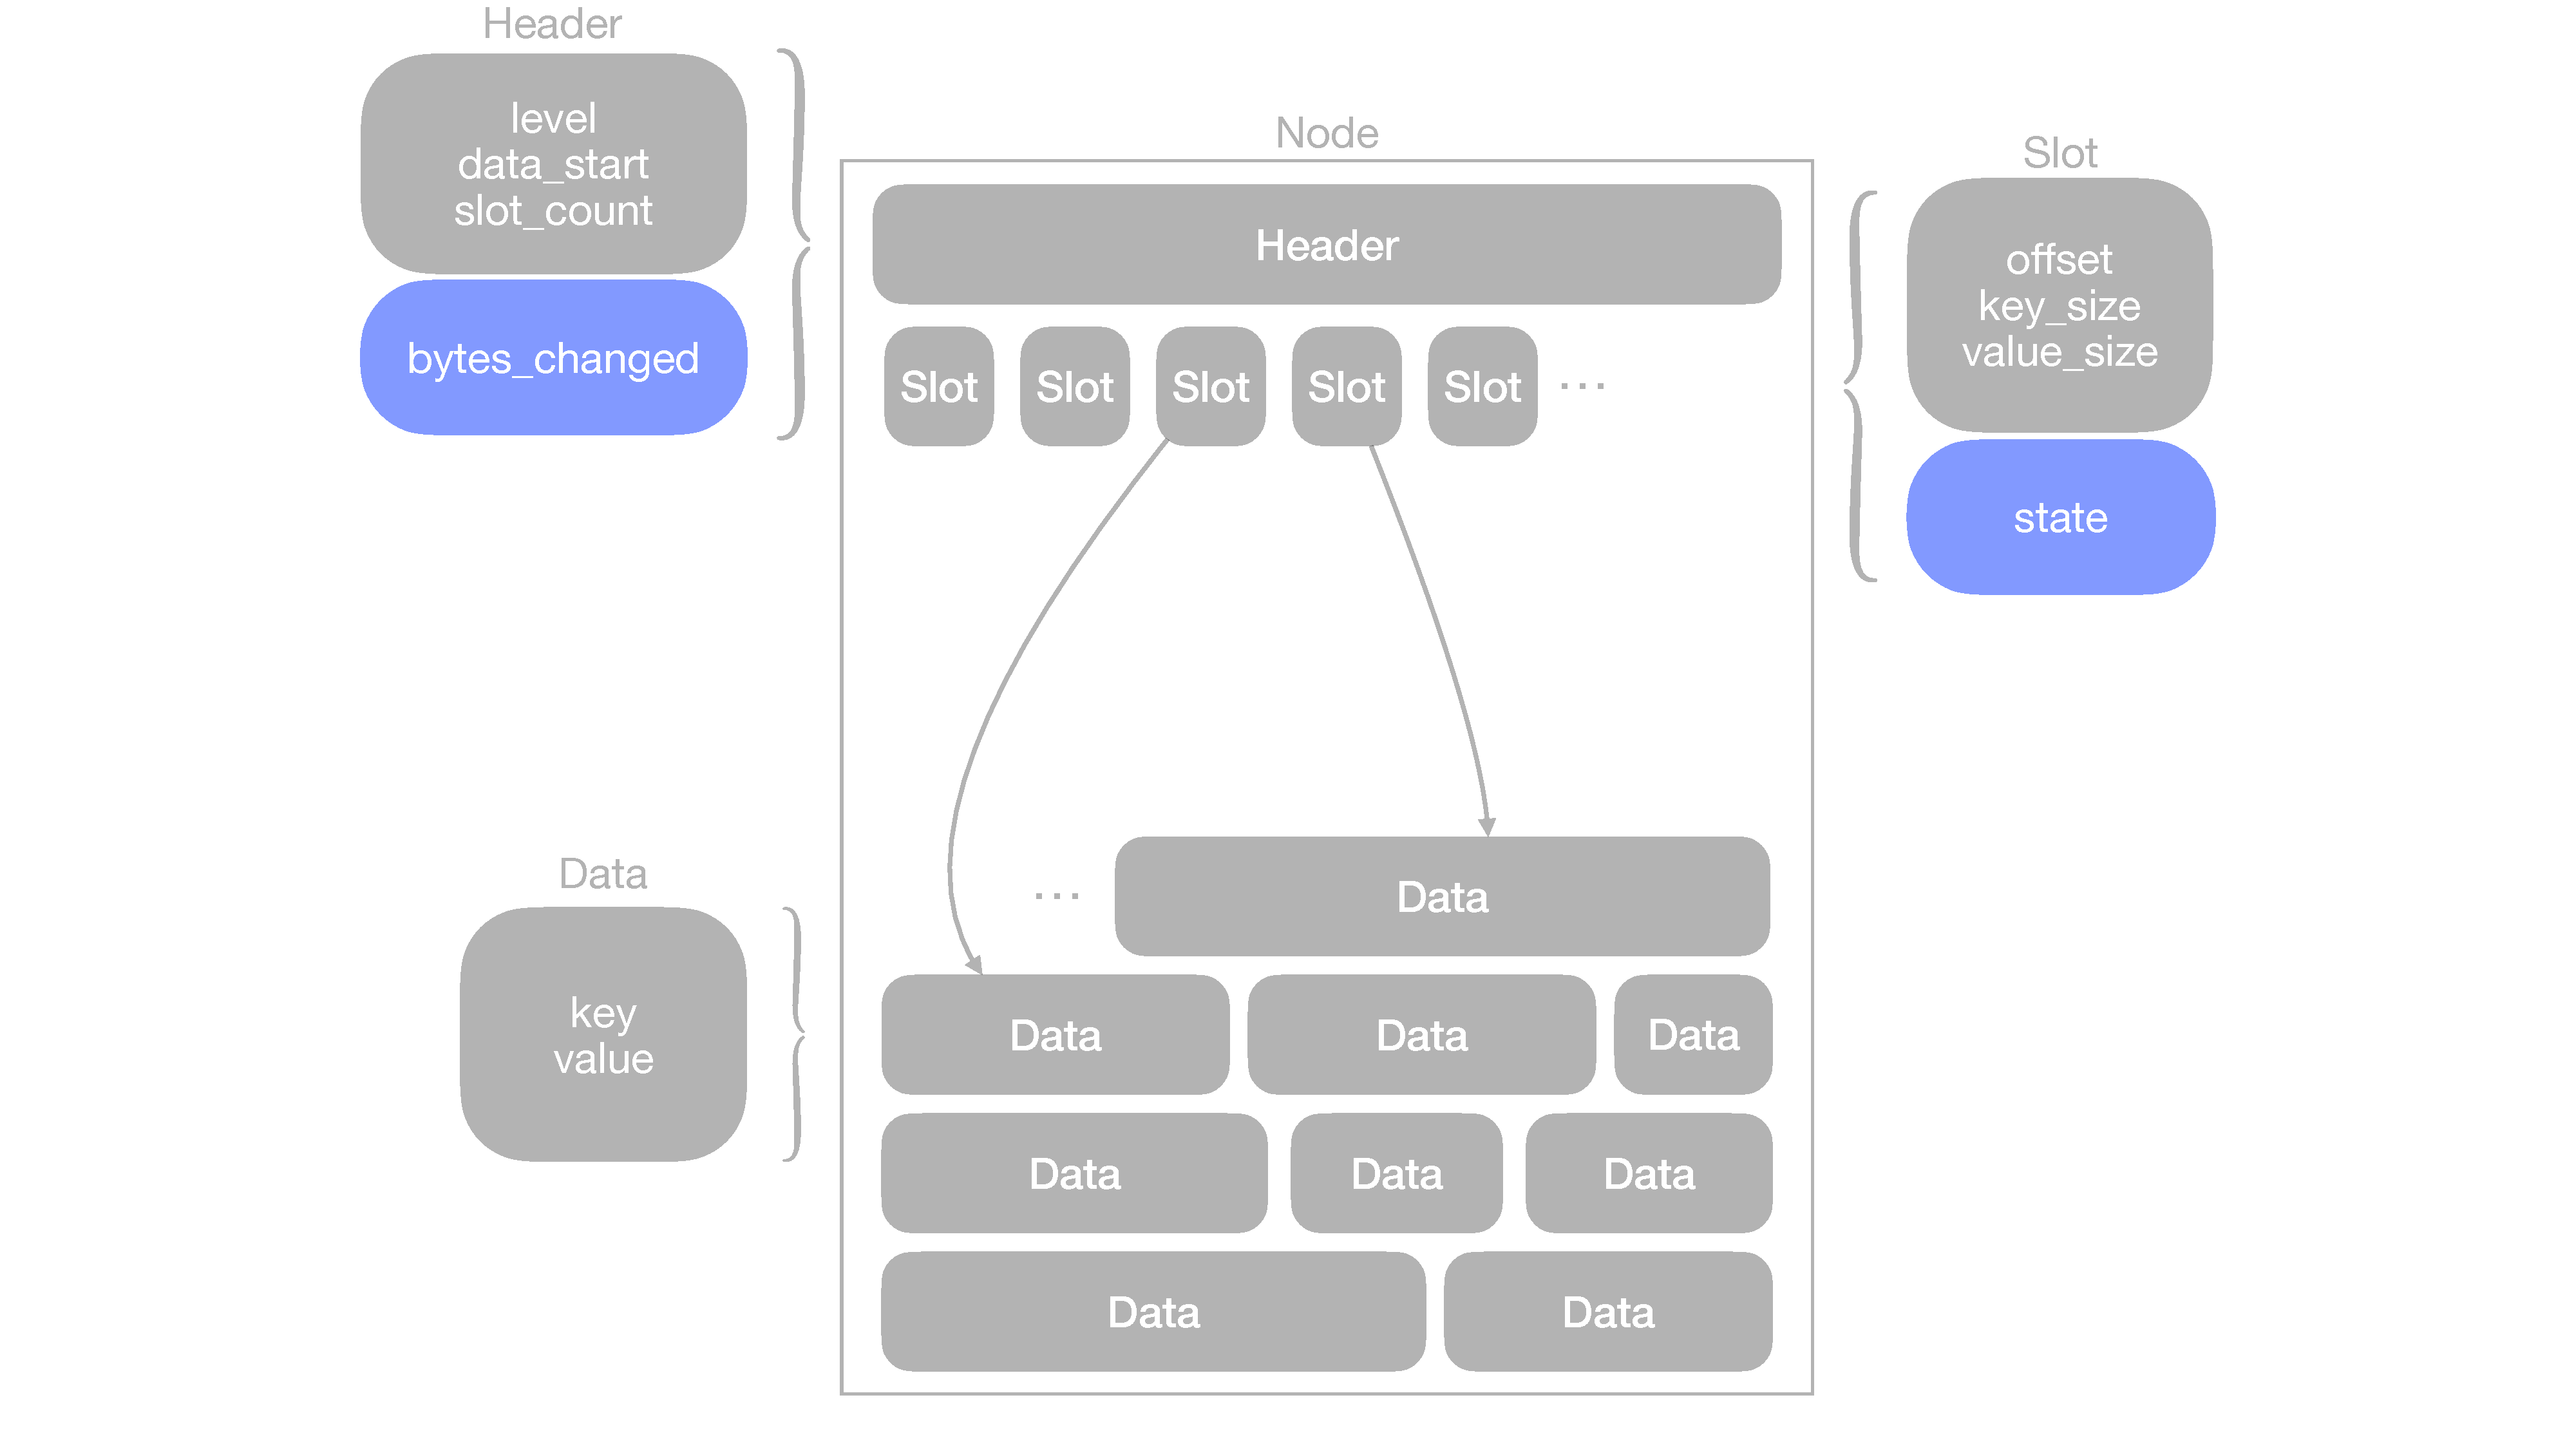
\includegraphics[width=1\textwidth]{figures/b_tree_with_tracking.pdf}
  \caption{A B-Tree with tracking enabled. The header is extended by a \texttt{bytes\_changed} field to track the degree of write amplification on the page. Each slot is extended by a \texttt{state} field to track whether the corresponding entry is \texttt{Unchanged}, \texttt{Inserted}, \texttt{Updated} or \texttt{Deleted}.}
  \label{fig:b-tree-with-tracking}
\end{figure}

\subsubsection*{Delta Tree}
The Delta Tree is responsible for storing and applying the changes made to the B-Tree nodes.
It is also a B-Tree but templated on a \ac{PID} as \texttt{KeyT} and a variable-sized \texttt{Delta} array as \texttt{ValueT}.

The \texttt{Delta} array stores the changes made to the corresponding page in the B-Tree.
A \texttt{Delta} array can contain either \texttt{InnerNodeDelta}s or \texttt{LeafDelta}s.
\texttt{InnerNodeDelta}s represent changes to inner nodes, therefore they store keys and \ac{PID} changes.
\texttt{LeafDelta}s represent changes to leaf nodes, therefore they store keys and \ac{TID} changes.

Each \texttt{Delta} array stores the \texttt{slot\_count} of the corresponding page in the B-Tree at the time of eviction.
For \texttt{InnerNodeDelta}s we additionally store the \texttt{upper} child \ac{PID}.
We do not need to store the level of the node, as a page never changes its level. 
Therefore, we can retrieve this information from the B-Tree when extracting or applying deltas.

After extracing and storing the \texttt{Deltas} of a B-Tree node in the Delta Tree, we can discard the node's page from the buffer manager without writing it to storage.
When the node is loaded from storage again, we can apply the stored \texttt{Deltas} to reconstruct the state of the node at the time of eviction.
In \autoref{sec:algorithms} we elaborate how we can reconstruct the state of a node from the information stored in the Delta Tree together with the disk-state of the node.

\subsection*{Database}
Our database class ties all components together.
It owns the buffer manager, the index and the slotted pages.
It exposes a simple key-value interface to the user, allowing to insert, update, delete and lookup tuples by keys.
The class is templated on the key type \texttt{KeyT} and the index type \texttt{IndexT}.
For simplicity, we only support a single table and a single \texttt{uint64\_t} value in our implementation.
Through the \texttt{IndexT} template parameter, the user can choose between a standard B-Tree or a BBB-Tree as index structure.

Whenever a user requests an operation, the database class translates it into the corresponding operations on the index and the slotted pages.

\section{Algorithms}
\label{sec:algorithms}
In this section we describe the algorithms for the main operations of our BBB-Tree.
While most operations are similar to a standard B-Tree \cite{mdbs2024slides}, we describe how we extend them to support tracking changes and ensure that we do not loose any changes made to a node.
We then describe how we use the tracking information in the B-Tree nodes to extract deltas when evicting a node from memory and how we can reconstruct the state of a node when loading it from storage again.

% TODO: Check which of these is still correct by the end of this thesis.
We do not implement concurrency or node merges in our implementation and therefore do not describe them here.
However, all algorithms were implemented with concurrency in mind and therefore can be extended to support it by introducing locks when fixing nodes.

\begin{figure}[htbp]
  \centering
  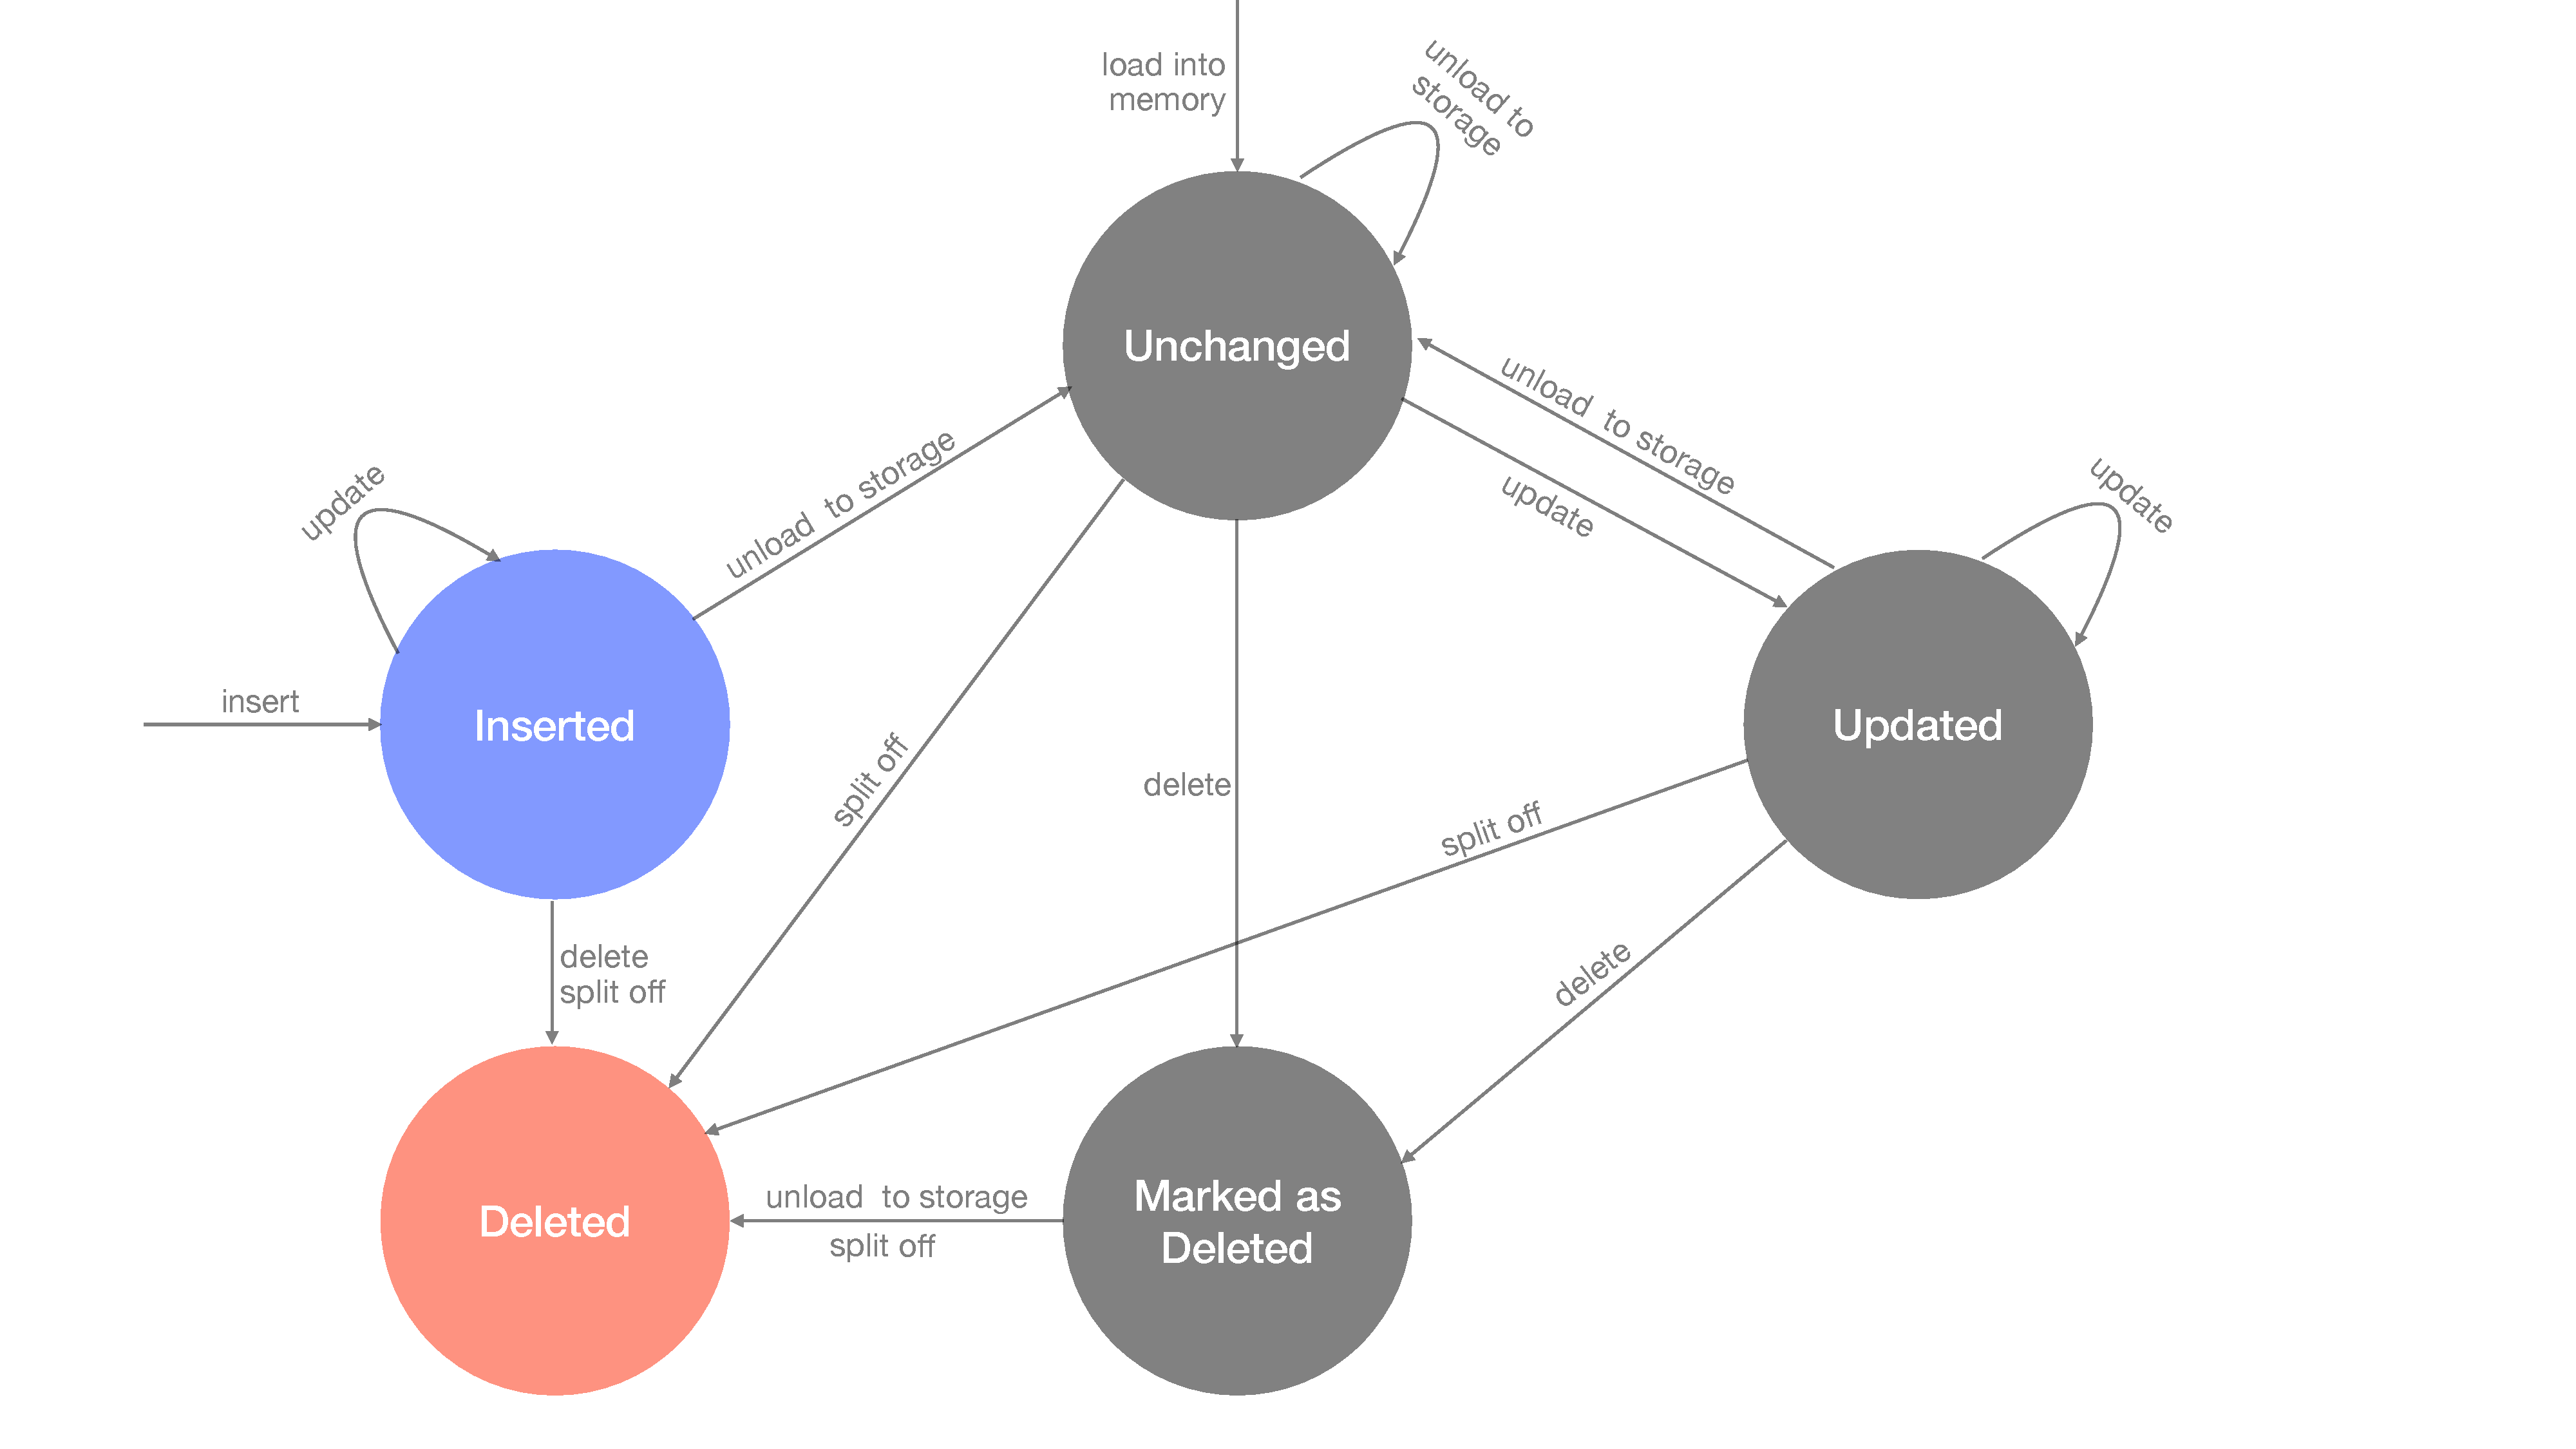
\includegraphics[width=1\textwidth]{figures/slot_states.pdf}
  \caption{The state machine of a slot's state. The state always resembles the delta of a slot in comparison to its image on disk. Therefore, every slot starts in the \texttt{Unchanged} state when being loaded from memory. A slot's lifetime starts with an insertion (highlighted in blue). Its lifetime ends when the slot is deleted (highlighted in red). When a page is unloaded back to storage, all \texttt{Inserted} and \texttt{Updated} slots are reset to \texttt{Unchanged} state. A slot marked as \texttt{Deleted} is actually deleted from the node once the page is unloaded.}
  \label{fig:slot-states}
\end{figure}

\subsection*{Lookup}
A lookup operation is straightforward in a BBB-Tree, we merely perform a standard B-Tree lookup.
We first access the root node and traverse the tree down to the leaf level, following the appropriate child pointers based on the key being looked up.
We always perform binary search within a node to find the appropriate slot. 
Once we reach the leaf level, we perform a final binary search to find the key.
If the key is found, we return the corresponding value, the \ac{TID}.
Since we return an \texttt{std::optional<ValueT>}, we can also indicate that the key was not found by returning an empty optional \texttt{nullopt}.

\inlinesection{Tracking.} 
Since we do not modify any nodes during a lookup, we do not need to update any tracking information.

\subsection*{Insert}
To perform an insertion, we first traverse the tree down to the appropriate leaf node as described in the lookup operation.

Possibly, the leaf node does not have enough space to accommodate the new entry.
In this case, we need to split the node first (see Split~\ref{subsec:split}).
Once we have an appropriate leaf node with enough space, we insert the new entry into the node.

Since we want to perform binary search within the node, we keep the slots sorted by key.
Therefore, we search for the \texttt{lower\_bound} of the new key to find the appropriate position in the slot array to insert the new slot.
We then shift all slots after the insertion position by one to make space for the new slot.
We then insert the new slot and the corresponding key and value into the data segment.

The property that slots are always sorted by key is important for the following algorithms.

\inlinesection{Tracking.} 
When inserting a new entry into a node, we need to update the tracking information accordingly.
Firstly, we increase the \texttt{bytes\_changed} field in the header by the size of the new entry and the size of the new slot.
Secondly, we set the \texttt{state} field of the new slot to \texttt{Inserted}.

A new slot always starts in the \texttt{Inserted} state, as it does not exist on disk (see \autoref{fig:slot-states}).
Any subsequent updates to this slot do not change this state, as to the disk image it is still a new slot.
During delta extraction, we simply store the latest key and value of this new slot.
If the new entry is deleted again before the page is evicted, we can simply discard the slot and do not need to store any delta for it.
To the disk image, it is as if the entry was never inserted.

\subsection*{Update}
In this operation, we only allow updating the value of an existing entry, not the key.
A key update is equivalent to a delete followed by an insert.

To perform an update on a value, we first traverse the tree down to the appropriate leaf node as described in the lookup operation.
Once we reach the leaf level, we perform binary search to find the slot with the given key.
If the key is found, we update the corresponding value in the data segment.
For simplicity, we assume that the new value has the same size as the old value.

In theory, we could translate all updates into a delete followed by an insert.
Since the delete operation loads all pages into memory already, the insert operation would not require any additional page loads (unless we require a node split).
However, if we delete an entry, we need to keep the entry in the node as a tombstone until the page is written back to storage (see Delete~\ref{subsec:delete}).
This would reduce the space available in the node for new entries, impacting the fanout of the tree.
However, one of our design goals is to minimize the performance impact on the B-Tree.
During node splits, for example, we must update the child pointers of the entries in the parent node (see Split~\ref{subsec:split}).
Therefore, we track updates separately to conserve space in the nodes.

\inlinesection{Tracking.} 
When updating an existing entry in a node, we increase the \texttt{bytes\_changed} field in the header by the size of the entry only if the entry was previously unchanged.
If the entry was previously marked as \texttt{Inserted}, we do not increase the \texttt{bytes\_changed} field, as we have already accounted for it.

We then set the \texttt{state} field of the slot to \texttt{Updated} if it was previously \texttt{Unchanged}.
If the slot was previously marked as \texttt{Inserted}, we do not change its state, as to the disk image it is still a new slot.

\subsection*{Delete}
\label{subsec:delete}
To perform a delete operation, we would first traverse the tree down to the appropriate leaf node as described in the lookup operation.
We then perform binary search to find the slot with the given key.
If the key is found, we remove the slot from the array and the corresponding entry from the data segment.
We do not reclaim the space in the data segment eagerly on every deletion.
Instead, we compactify lazily. 
For example, during a node split we remove half of the slots and their data, justifying a compactification.

\inlinesection{Tracking.}
% TODO: check if this is still correct.
While we do not implement deletion tracking in our current implementation, we describe how we would implement it here for completeness.
When deleting an existing entry in a node, we increase the \texttt{bytes\_changed} field in the header by the size of the entry and the size of the slot only if the entry was previously unchanged.
When it was previously inserted, we decrease the \texttt{bytes\_changed} field, since the insert never happened from the perspective of the disk image of the node.
For the same reason, we only actually delete the slot and entry if it was also inserted since its last write to storage.
In any other case, we cannot immediately delete the slot.
This is, because we must indicate the deletion to the Delta Tree.
The entry exists on disk and without an entry to track the deletion, we would not be able to create a delta for it.
When loading the node again from storage, the deleted entry would reappear.
Therefore, we set the \texttt{state} field of the slot to \texttt{Deleted} instead.
Only when the page is written to disk, we actually delete all slots marked as \texttt{Deleted} from the node.

\subsection*{Split}
\label{subsec:split}
When a leaf node does not have enough space to accommodate a new entry, we need to split the node first.
To address the possibility of concurrent splits in the future, we use a restart mechanism.

We first traverse the tree down to the appropriate leaf node as described in the lookup operation.
However this time, we keep track of the path taken down the tree and keep the pages fixed in memory.
Once we reach the leaf level, we check whether the node has enough space to accommodate the new entry in the current iteration.
Firstly, this is necessary in a concurrent setting, as another thread might have split the node in the meantime.
Secondly, this is necessary, because splitting a leaf node once might not be enough to accommodate the new entry when supporting variable-sized entries.
For example, we could have a new entry that is as large as the entire node.
In that case, we would need to split the node multiple times until we reach an empty node.

If the leaf has enough space, we return.
Otherwise, we split the node.
We allocate a new sibling node and move half of the entries from the current node to the sibling.
Then, the new \ac{PID} of the sibling and the new fence key are propagated up the tree.
The new fence key is the largest key in the left node after the split.
We can move upwards now, since we locked the path exclusively when traversing down the tree.
If the parent node does not have enough space to accommodate the new fence key and child pointer, we need to split the parent node as well.
We repeat this process until we reach a node that has enough space in an upwards motion.
Should we reach the root node and it does not have enough space, we create a new root node, increasing the tree's height by one.
Once a node has enough space, we can insert the new entry and move back down the tree to insert the respective entries on each level.
Again, we might need to split nodes on the way down again, since we support variable-sized keys.
Therefore, we can repeatedly move down and up the tree until we reach the leaf level again.
When reaching the leaf level, we repeat the process until the leaf has enough space to accommodate the new entry.

Finally, we insert the new entry into the leaf node.

Some implementations use "safe" inner pages that always have enough space to accommodate a new entry \cite{mdbs2024slides}.
This simplifies the split operation, as we never have cascading splits that need to propagate up the tree.
However, this is limited to fixed-sized keys.
With variable-sized keys, we cannot know how much space we need to reserve in the inner nodes to accommodate a new fence key.

When creating a new node, we always write it out to storage on eviction.
This is because new nodes carry enough information to justify the write.
Also, it greatly simplifies tracking, since we can express all deltas as slot changes.

After splitting a node, we compactify the node to reclaim space from deleted slots and to defragment the data segment.

\inlinesection{Tracking.}
When splitting a node, we delete half of the slots from the perspective of the current node.
For each deleted slot, we increase the \texttt{bytes\_changed} field in the header by the size of the entry and the size of the slot only if the entry was previously unchanged.
If the entry was previously inserted or updates, those bytes were already accounted for.
The \texttt{bytes\_changed} field is only an approximation of the actual degree of change on the page.
This is, because we can change the same bytes multiple times by deleting and inserting slots.
For example, we can split a node, deleting half of the slots, and then insert new slots again.
We do not aim to account for every single byte change, but rather to get a rough estimate of the degree of change on the page.
This allows us to make informed decisions whether a write-out is justified at the time of eviction.

As we discussed in the delete operation (see Subsection~\ref{subsec:delete}), we usually cannot actually delete the slots from the node, as we need to track the deletion as a delta to ensure that we do not make entries reappear when loading the node from storage again.
However, we cannot mark the slots as \texttt{Deleted}, since that would keep the data in the node and therefore not free up any space, negating the purpose of a node split.
For node splits we use a different approach.
Due to the fact that slots are always sorted by key and we always split the node in half, we can use the \texttt{slot\_count} field in the header to determine which slots are still part of the node and which slots were split off.
Therefore, we do not need to keep any tracking information for the split off slots.
Instead, we store the \texttt{slot\_count} of the node at the time of eviction in the corresponding \texttt{Delta} array.
When applying deltas to a node, we can use this information to determine which slots are still part of the node and which slots were split off.
This way, we can discard split off nodes, freeing up space for new entries.
To the new sibling node, the moved over slots are marked as \texttt{Inserted}.

As described above, when a child node splits, we need to insert the new fence key and new child pointer into the parent node.
The key that is already present in the parent node remains unchanged, as it still forms the upper bound of that range.
However, it is not the upper bound of the new sibling node. Therefore we perform an update on the existing slot, changing the child pointer to the new sibling node.
The tracking information for that node changes according to the update operation described above.
The new fence key is now the upper bound for the split node. 
Therefore, we insert a new slot into the parent node with the new fence key and the old child pointer.
The tracking information for that node changes according to the insert operation described above.

\subsection*{Compactification}
To reclaim free space, we compactify a node by defragmenting the data segment.
Fragmentation in a node occurs through deletions, since we do not reclaim the space in the data segment eagerly.
This would require moving possibly all entries in the data segment and updating the corresponding slots.
This would be an expensive operation to perform on every deletion.
Instead, we perform compactification lazily, for example after a node split.
After a node split, half of the slots are removed from the node, freeing up a significant amount of space.
More importantly, we split a node in particular to free up space for new entries.

First, we collect pointers to all slots that still point to valid entries.
We also collect slots marked as \texttt{Deleted}, as we need to keep them in the node until the page is written back to storage to track the deletion as a delta.
We then sort them by their offset in the data segment, starting with the highest offset.
Then, we move the entries to the end of the data segment, updating the corresponding offsets in the slot accordingly.
Finally, we update the header to point to the new start of the data segment.

\inlinesection{Tracking.}
Since compactification only moves entries around in the data segment, we do not change the node logically.
Therefore, we do not change any tracking information.
However, compactification is an expensive operation and reclaiming space is important to keep the fanout of the tree high.
We would like to maintain the space gains from compactification also after discarding the page and loading it again from memory.
Therefore it makes sense to always write out a page after a node split, as a node split usually carries enough information through its structural changes to justify the write.
If we require more than 50\% change on the page to perform a write-out, this would be a given, since we change half of the node during node splits.
% TODO: Check if this is still correct by the end of the thesis:
In \ref{chap:evaluation} we will see that requiring a degree of change of even less than 50\% is a reasonable threshold to perform a write-out.

\subsection*{Eviction}
When the buffer manager evicts a B-Tree's node from memory, it evokes the injected Delta Tree.
It needs to decide whether to write out the page to storage or not.
To that end, we calculate the degree of change, by comparing the \texttt{bytes\_changed} field in the header to the size of the node.
\[degree\_of\_change = bytes\_changed / page\_size\]
The Delta Tree is passed a threshold parameter $wa\_threshold$ between 0 and 100.
It determines the minimum $degree\_of\_change$ required to justify a write-out of the page.

\subsection*{Resetting Deltas}
If $degree\_of\_change > wa\_threshold$, we write the page to storage. 
In that case, we scan the slot array of the node and reset all tracking information:
We set all slots to \texttt{Unchanged} state.
We remove all \texttt{Deleted} slots from the node, as they are now actually deleted from the disk image of the node.
We set the \texttt{bytes\_changed} field in the header to 0.
Finally, we erase any corresponding deltas for this page from the Delta Tree, as they are now obsolete.
We can perform a standard B-Tree deletion.
We indicate to the buffer manager to continue writing the page to storage.

\subsection*{Extracting Deltas}
If $degree\_of\_change \leq wa\_threshold$, we extract all deltas from the node and store them in the Delta Tree.
We scan the slot array of the node and for each slot that is not \texttt{Unchanged}, we create a corresponding delta.
The resulting delta array is then stored in the Delta Tree with the node's \ac{PID} as key.
This is done with a standard B-Tree insertion.
Finally, we indicate to the buffer manager to discard the page without writing it to storage.

\subsection*{Applying Deltas}
When the buffer manager loads a B-Tree's node from storage, it invokes the injected Delta Tree to apply any stored deltas to the node.
We first check whether there are any deltas stored for the node's \ac{PID} in the Delta Tree.
If not, we are done.
Otherwise, we apply the deltas to the node.
In the end we cut off any slots that were split off during a node split by using the stored \texttt{slot\_count} in the delta array.
Since we apply inserts and updates before cutting off split slots, we can ensure that we do not let any entries reappear that were actually split off. 
This must be correct, since we only stored deltas for slots that are still part of the node at eviction time.
Everything beyond the stored \texttt{slot\_count} was split off and therefore cannot be part of the node.

However, when applying deltas to a node, we might exceed the node size temporarily.
For example, we could have a node that is full on disk. 
In memory it had been split and then some insertions followed. 
When applying the deltas to the full node, we would exceed the node size, since we perform the insertions before cutting off the split slots.

To address this, we allow exceeding the node size temporarily when a node becomes full while applying deltas
After cutting off split slots, we compactify the node and shrink it back to its original size.

We keep the deltas in the Delta Tree after applying them.
This allows us to keep the page in a clean state should it be evicted again without any changes.
We can simply discard the page, without needing to extract and store the deltas again.

\section{Testing}
All components of our system are covered by unit tests.
We used the Google Test framework to write and run our tests.
We tested the buffer manager, the slotted pages, the B-Tree, and the BBB-Tree separately.
We also wrote integration tests to test the interaction between the components.

% \section{Challenges and Trade-offs}
% TODO: Maybe add this section.
% Want to keep compactification. Otherwise we could put changes in delta tree and then do unneccessary splits because the node does not have enough space after applying the changes again witout compactification.

% Locking a node to protect recursive evictions.

% After a node split we generally want to write out the page because it carries a lot of information and compactification work savings.
% Problem of recursive calls to the Delta Tree. Locking the tree when operating on it. Otherwise it could access uninitialized nodes during splits for example.

% Notion of time.

% Scanning Deltas when evicting VS. keeping the DeltaTree up to date during manipulation of the B-Tree.

% What happens when a new node is created? (see Storyline)

% What happens on destruction? (see Storyline)

% Size of the operation state field in the slot. 2 bit should be enough.

% Recursive eviction calls to Delta Tree. Can access unintialized root node.

% Want to keep Deltas in the tree after applying them to be able to just throw them away when only reading. Less changes to the tree
% However: what do we do with stale deltas? Do we want to apply the at some point?
% We have an incentive to keep the Delta Tree small to batch changes more effectively. Therefore we can evict changes from the Delta Tree if they have not been used for a while.
% Also we should only track small changes. If a page has a lot of changes, it is better to write it out and not track it anymore.

% When deltas become too big they might not fit a single leaf node in the Delta Tree anymore. That's a limitation. All pages are of same size.

% Deltas have lower fanout because of variable sized values. Therefore we have a taller tree and more IOs to access a delta.

